\documentclass[aspectratio=43,11pt]{beamer}

% ================================================================
% Presentación de TP5 — Dinámica peatonal, capas de elusión (72.25, ITBA).
% Estilo heredado de TP3/presentacion/template_presentacion_tp3.tex (D27).
% Compilar con: latexmk -pdf -outdir=generated presentacion_tp5.tex
% Símbolos nuevos: definir en texto + marca visual la primera vez (ver DEFINICIONES.md §5).
% ================================================================

% ----------------------------------------------------------------
% REVISAR A MANO antes de aceptar (corrección real de TP2: un label
% de eje sobrecargado "suena a eje nombrado por la IA"). Convención
% acordada para TODAS las figuras de esta presentación:
%   eje temporal .......... t [s]
%   paso temporal ......... Δt [s]
%   error cuadrático medio  ECM
%   energía relativa ...... E/E₀
%   error de energía ...... ε_E
%   cantidad de partículas  N
%   fracción usada ........ F_u
%   tiempo al 90% ......... ⟨t₉₀⟩ [s]
%   rapidez ............... v [m/s], f(v)
%   densidad .............. ρ [m⁻²]
% Nada de paréntesis explicativos ni unidades del modelo entre
% corchetes. Si un label no entra en dos o tres símbolos, está mal.
%
% TAMAÑO DE FUENTE (corrección real de TP2: "los tamaños de fuente de
% las figuras son ilegibles"): la letra dentro de cada figura tiene que
% ser comparable a la del resto de la diapositiva. Si no se lee
% proyectada, está mal, sea cual sea el tamaño en puntos.
%
% NUNCA un título adentro del área graficada: eso va en el
% \frametitle. Los parámetros fijos van en el \parambox del costado,
% nunca repetidos en cada entrada de leyenda.
%
% TEXTO (D27): lo escribe una persona a partir de la figura. Los
% títulos de cada diapositiva son provisorios; los recuadros grises con
% "Sxx — ..." marcan qué va (DEFINICIONES.md §3) y se reemplazan.
% ----------------------------------------------------------------

\usepackage[T1]{fontenc}
% "provide=*" permite compilar también en instalaciones mínimas de TeX Live.
\usepackage[provide=*,spanish]{babel}
\usepackage{lmodern}
\usepackage{amsmath,amssymb,bm}
\usepackage{graphicx}
\usepackage{tikz}
\usetikzlibrary{arrows.meta,calc,positioning,decorations.pathmorphing}
% Para controlar leftmargin/itemsep/topsep del itemize angosto de \parambox
% (0.27\textwidth) -- el itemize default de beamer queda con demasiado
% margen y espaciado para una caja tan chica.
\usepackage{enumitem}
% enumitem reemplaza el símbolo de beamer por uno vacío: sin esto los itemize
% sin label explícito (ej. Conclusiones) salen sin viñeta.
\setlist[itemize]{label=\textcolor{TPBlue}{$\bullet$}}

% ---------- Colores ----------
\definecolor{TPBlue}{HTML}{3939B5}
\definecolor{TPBlueDark}{HTML}{29298A}
\definecolor{TPBlack}{HTML}{050505}
\definecolor{TPNavGray}{HTML}{858585}
\definecolor{TPLight}{HTML}{E9E9F2}
\definecolor{TPPlaceholder}{HTML}{F4F4F7}
\definecolor{TPFresca}{HTML}{2E5FD0}
\definecolor{TPUsada}{HTML}{C0392B}

\setbeamercolor{normal text}{fg=black,bg=white}
\setbeamercolor{structure}{fg=TPBlue}
\setbeamercolor{frametitle}{fg=white,bg=TPBlue}
\setbeamercolor{itemize item}{fg=TPBlue}
\setbeamercolor{itemize subitem}{fg=TPBlue}
\setbeamercolor{title box}{fg=white,bg=TPBlue}
\setbeamercolor{databox title}{fg=white,bg=TPBlueDark}
\setbeamercolor{databox body}{fg=black,bg=TPLight}
\setbeamercolor{algorithm box}{fg=black,bg=white}
\setbeamercolor{headline navigation}{fg=TPNavGray,bg=TPBlack}
\setbeamertemplate{items}[circle]
\setbeamertemplate{navigation symbols}{}

\setbeamerfont{frametitle}{size=\Large,series=\mdseries}
\setbeamerfont{normal text}{size=\normalsize}
\setbeamerfont{itemize/enumerate body}{size=\normalsize}
\setbeamerfont{itemize/enumerate subbody}{size=\small}

% ---------- Metadatos ----------
\title{Trabajo Práctico Nro. 5: Dinámica Peatonal, Capas de Elusión}
\subtitle{72.25 - Simulación de Sistemas}
\author{%
  Federico Ignacio Ruckauf\texorpdfstring{\textsuperscript{1}}{1}
  \and Federico Spivak Fontaiña\texorpdfstring{\textsuperscript{2}}{2}
  \and Lorenzo Chiossone\texorpdfstring{\textsuperscript{3}}{3}%
}
\institute{Instituto Tecnológico de Buenos Aires}
\date{2026 2C --- Grupo N.º 02}
\hypersetup{pdftitle={SdS\_TP5\_2026Q2G02CS\_Presentación}}

% Animaciones (links a YouTube/Vimeo; completar cuando estén subidas).
\newcommand{\animacionURL}{https://youtu.be/PENDIENTE-ab}           % evento 16: real, A y B
\newcommand{\animacionSinCapaURL}{https://youtu.be/PENDIENTE-sincapa} % evento 16: real, sin capa y A
\newcommand{\animacionRecorteURL}{https://youtu.be/PENDIENTE-recorte} % evento 16: recorte al tramo frontal
\newcommand{\animacionLadoURL}{https://youtu.be/PENDIENTE-lado}       % evento 12: A elige el lado de cruce contrario al real

% Números del piloto aún provisorios: salen en naranja. Poner \provisoriofalse al cerrar.
\newif\ifprovisorio\provisoriofalse
\definecolor{TPProv}{HTML}{D9730D}
\newcommand{\prov}[1]{\ifprovisorio\textcolor{TPProv}{#1}\else #1\fi}
\newcommand{\pend}{\textcolor{TPUsada}{\textbf{[pend.]}}}

% Si existe logo_itba.png o logo_itba.pdf junto al .tex, se inserta.
\newcommand{\institutionlogo}{%
  \IfFileExists{logo_itba.pdf}{\includegraphics[height=0.75cm]{logo_itba.pdf}}{%
    \IfFileExists{logo_itba.png}{
\includegraphics[height=0.75cm]{logo_itba.png}}{%
      \fbox{\scriptsize LOGO DE LA INSTITUCIÓN}%
    }%
  }%
}

% ---------- Barra superior por sección ----------
% Rangos de diapositivas:
% Introducción 2--5 (incluye Modelo) | Implementación 6--7
% Simulaciones 8--11 | Resultados 12--19 | Conclusiones 20--22
% Anexo 24--37. El cierre (23) queda fuera de la barra.
% Cada rango incluye su \sectiondivider como primera diapositiva del
% bloque. Si se agregan o quitan diapositivas hay que renumerar estos
% rangos a mano.
\newcount\TPNavDot

% Asegúrate de tener \usepackage{pgffor} en tu preámbulo (Beamer ya lo incluye)
\newcommand{\navdots}[2]{%
  \foreach \n in {#1,...,#2} {%
    \ifnum\insertframenumber=\n\relax
    \raisebox{0.45mm}{{\color{white}\fontsize{6}{6}\selectfont$\bullet$}}%
    \else
      \raisebox{0.45mm}{{\color{TPNavGray}\fontsize{7}{7}\selectfont$\circ$}}%
    \fi
    \ifnum\n<#2\relax
    \kern0.60mm
    \fi
  }%
}


\newcommand{\navblock}[4]{%
  % #1 ancho, #2 nombre, #3 inicio, #4 fin
  \makebox[#1\paperwidth][c]{%
    \parbox[c][0.62cm][c]{#1\paperwidth}{%
      \centering
      \ifnum\insertframenumber>1
        \ifnum\insertframenumber<#3
          {\color{TPNavGray}\scriptsize\strut #2}%
        \else
          \ifnum\insertframenumber>#4
            {\color{TPNavGray}\scriptsize\strut #2}%
          \else
            {\color{white}\scriptsize\strut #2}%
          \fi
        \fi
      \else
        {\color{TPNavGray}\scriptsize\strut #2}%
      \fi
      \par\vspace{-0.55mm}
      \navdots{#3}{#4}%
    }%
  }%
}

% Fila de navegación por secciones -- factorizada para no duplicarla
% entre las dos ramas de \TPheadline (con y sin franja de relleno).
\newcommand{\TPnavrow}{%
  \makebox[\paperwidth][l]{%
    \navblock{0.14}{Introducción}{2}{5}%
    \navblock{0.155}{Implementación}{6}{7}%
    \navblock{0.135}{Simulaciones}{8}{11}%
    \navblock{0.145}{Resultados}{12}{19}%
    \navblock{0.135}{Conclusiones}{20}{22}%
    \navblock{0.29}{Anexo}{24}{37}%
  }%
}

% La franja azul de relleno (para diapositivas sin título, ej.
% \sectiondivider) NUNCA debe cambiar la altura TOTAL del headline: si se
% suma como una caja extra arriba de la altura de la barra de navegación
% normal, el headline queda 0.05cm (~1.42pt) más alto que en las
% diapositivas con título, y LaTeX no tiene margen para absorberlo en los
% frames centrados verticalmente ([c], o con \vfill como portada/cierre)
% -- produce "Overfull \vbox (1.42271pt too high)" y una línea residual
% visible en el borde superior. Por eso la franja le resta exactamente lo
% mismo que ocupa al "dp" de la barra de navegación (0.28cm -> 0.23cm):
% el total (barra + franja) da siempre 0.78cm, igual que una diapositiva
% con título.
\setbeamertemplate{headline}{%
  \leavevmode
  \ifdefempty{\insertframetitle}{%
    \begin{beamercolorbox}[wd=\paperwidth,ht=0.50cm,dp=0.23cm]{headline navigation}%
      \TPnavrow
    \end{beamercolorbox}%
    \par\nointerlineskip
    \begin{beamercolorbox}[wd=\paperwidth,ht=0.05cm,dp=0cm]{frametitle}\end{beamercolorbox}%
  }{%
    \begin{beamercolorbox}[wd=\paperwidth,ht=0.50cm,dp=0.28cm]{headline navigation}%
      \TPnavrow
    \end{beamercolorbox}%
  }%
}

\setbeamertemplate{frametitle}{%
  \nointerlineskip
  \begin{beamercolorbox}[wd=\paperwidth,ht=0.74cm,dp=0.12cm,leftskip=0.35cm]{frametitle}
    \usebeamerfont{frametitle}\insertframetitle
  \end{beamercolorbox}
}

\setbeamersize{text margin left=0.55cm,text margin right=0.55cm}

% Pie mínimo con número de diapositiva.
\setbeamertemplate{footline}{%
  \leavevmode
  \hbox{\begin{beamercolorbox}[wd=\paperwidth,ht=0.20cm,dp=0.10cm,rightskip=0.18cm]{normal text}
    \hfill{\color{TPNavGray}\tiny\insertframenumber/\inserttotalframenumber}
  \end{beamercolorbox}}
}

% ---------- Componentes reutilizables (heredados de TP2/TP3) ----------
\newcommand{\sectiondivider}[1]{%
  \begin{frame}[c]{}
    \makebox[\linewidth][c]{%
      \begin{beamercolorbox}[wd=0.56\paperwidth,ht=0.55cm,dp=0.15cm,center]{frametitle}
        \large #1
      \end{beamercolorbox}%
    }
  \end{frame}
}

\newcommand{\placeholder}[2][4.4cm]{%
  \begingroup
    \setlength{\fboxsep}{0pt}%
    \setlength{\fboxrule}{0.45pt}%
    \fcolorbox{TPNavGray}{TPPlaceholder}{%
      \parbox[c][\dimexpr#1-2\fboxrule\relax][c]{%
        \dimexpr\linewidth-2\fboxrule\relax}{%
        \centering\color{TPNavGray}\small #2}%
    }%
  \endgroup
}

\newcommand{\maybeimage}[3]{%
  \IfFileExists{#1}{\includegraphics[width=\linewidth,height=#2,keepaspectratio]{#1}}{%
    \placeholder[#2]{#3\\[2mm]\nolinkurl{#1}}%
  }%
}

% Ambas versiones muestran debajo un enlace visible a YouTube.
% En la versión YouTube, además, la propia imagen funciona como enlace.
\newcommand{\videooimagen}[4]{%
  \begin{minipage}{\linewidth}
    \centering
    \ifdefined\versionyoutube
      \href{#3}{\maybeimage{#1}{#2}{#4}}%
    \else
      \maybeimage{#1}{#2}{#4}%
    \fi
    \par\vspace{1mm}
    % En vivo la URL no se ve, pero ocupa el mismo lugar: así el fotograma queda en la misma posición
    % que en el PDF de entrega y el video del PPTX lo tapa exacto.
    \ifdefined\versionvivo
      \phantom{{\scriptsize\nolinkurl{#3}}}%
    \else
      \href{#3}{{\color{TPBlue}\scriptsize\nolinkurl{#3}}}%
    \fi
  \end{minipage}%
}

% Caja de parámetros fijos, en la columna derecha (~28% del frame) --
% nunca repetidos dentro de la leyenda (corrección real de TP2). Lista de
% viñetas alineada a la izquierda (no centrada): el contenido se pasa como
% una secuencia de \item, ej. \parambox{\item A \item B \item C}.
\newcommand{\parambox}[1]{%
  \begin{beamercolorbox}[wd=\linewidth,sep=2mm]{databox body}
    % Alineada a la izquierda y sin cortes con guion: en columnas angostas el justificado dejaba huecos
    \small\raggedright\hyphenpenalty=10000\exhyphenpenalty=10000
    \begin{itemize}[label=\textcolor{TPBlue}{$\bullet$},leftmargin=3.2mm,labelsep=1mm,itemsep=1mm,topsep=0pt,parsep=0pt]
      #1
    \end{itemize}
  \end{beamercolorbox}%
}

% Una animación por diapositiva, con la caja de parámetros al costado.
% #1 imagen, #2 altura, #3 URL, #4 texto del placeholder, #5 parámetros fijos.
\newcommand{\animacionsimple}[5]{%
  \begin{columns}[T,onlytextwidth]
    \begin{column}{0.66\textwidth}
      \videooimagen{#1}{#2}{#3}{#4}%
    \end{column}
    \begin{column}{0.31\textwidth}
      \parambox{#5}%
    \end{column}
  \end{columns}%
}

% Diapositiva de resultados: figura a la izquierda (0.66) y, a la derecha,
% la caja de parámetros fijos y opcionalmente una imagen chica (fotograma
% de la animación o esquema) con su epígrafe.
% #1 figura, #2 altura, #3 texto del placeholder, #4 parámetros fijos,
% #5 imagen chica (vacío = sin imagen), #6 epígrafe de la imagen chica.
% Columnas 0.73 / 0.25 (antes 0.66 / 0.31): la figura queda lo más grande posible y la caja de
% parámetros, en columna a la derecha (pedido del grupo, 23/10).
\newcommand{\resultadofigura}[6]{%
  \begin{columns}[T,onlytextwidth]
    \begin{column}{0.73\textwidth}
      \centering
      \maybeimage{#1}{#2}{#3}%
    \end{column}
    \begin{column}{0.25\textwidth}
      \ifstrempty{#4}{}{\parambox{#4}\par\vspace{2mm}}%
      \ifstrempty{#5}{}{%
        \centering
        \maybeimage{#5}{3.2cm}{Imagen chica}\par
        {\scriptsize\color{TPNavGray}#6\par}%
      }%
    \end{column}
  \end{columns}%
}

\newenvironment{databox}[1]{%
  \begin{beamercolorbox}[wd=\linewidth,sep=1mm,center]{databox title}%
    #1
  \end{beamercolorbox}%
  \par\nointerlineskip
  \begin{beamercolorbox}[wd=\linewidth,sep=2mm]{databox body}%
}{%
  \end{beamercolorbox}%
}


% ================================================================
% PRESENTACIÓN TP5 — Problema 1 (el grupo no hace el Problema 2)
% BORRADOR para mostrar a la cátedra. Números del piloto con recorte D(45°) + compuerta X = 1,5 m.
% \prov pasa a naranja con \provisoriotrue; \pend = falta.
% ================================================================
\begin{document}

\begin{frame}{}
  \vspace{0.35cm}
  \makebox[\linewidth][c]{%
    \begin{beamercolorbox}[wd=0.91\linewidth,sep=3mm,center]{title box}
      \resizebox{0.92\linewidth}{!}{\strut\inserttitle}\par
      \vspace{1mm}{\large\insertsubtitle}
    \end{beamercolorbox}%
  }\par
  \vspace{0.35cm}
  \begin{center}
    {\small\insertauthor\par}\vspace{0.18cm}
    {\scriptsize
      \textsuperscript{1}\href{mailto:fruckauf@itba.edu.ar}{fruckauf@itba.edu.ar}\\[0.5mm]
      \textsuperscript{2}\href{mailto:fespivak@itba.edu.ar}{fespivak@itba.edu.ar}\\[0.5mm]
      \textsuperscript{3}\href{mailto:lchiossone@itba.edu.ar}{lchiossone@itba.edu.ar}\par}
    \vspace{0.13cm}{\small\insertinstitute\par}
    \vspace{0.35cm}{\large\insertdate\par}
    \vfill\institutionlogo
  \end{center}
\end{frame}

% ---------------- INTRODUCCIÓN ----------------
\sectiondivider{Introducción}

% 3 -- Introducción + SFM (Teórica 6, diapos 28, 29 y 31; Helbing 2000)
\begin{frame}{Dinámica peatonal: SFM sin fuerza social}
  \setlength{\abovedisplayskip}{2pt}\setlength{\belowdisplayskip}{2pt}
  \begin{itemize}\small
    \item Dos peatones que se cruzan de frente esquivan antes de chocar
    \item SFM sin fuerza social + \emph{capa de elusión}: la capa solo cambia la dirección deseada
  \end{itemize}
  \begin{columns}[T,onlytextwidth]
    \begin{column}{0.60\textwidth}
      {\small\textbf{Ecuación de movimiento}}
      \[ m\,\ddot{\mathbf{x}}_i = m\,\frac{v_d\,\mathbf{e}_i - \dot{\mathbf{x}}_i}{\tau} + \sum_{j:\,\varepsilon_{ij}<0} \mathbf{F}_G^{ij} \]
      {\small\textbf{Contacto}}
      \[ \mathbf{F}_G^{ij} = -k_n\,\varepsilon_{ij}\,\hat{\mathbf{n}} + k_t\,\varepsilon_{ij}\,\big((\mathbf{v}_i - \mathbf{v}_j)\cdot\hat{\mathbf{t}}\big)\,\hat{\mathbf{t}} \]
      {\small\textbf{Dirección deseada}}
      \[ \mathbf{e}_i = \begin{cases} \mathbf{e}_t = \dfrac{\mathbf{x}_f - \mathbf{x}_i}{|\mathbf{x}_f - \mathbf{x}_i|} & \text{sin capa} \\[2mm] \mathbf{e}_a & \text{con capa} \end{cases} \]
    \end{column}
    \begin{column}{0.37\textwidth}
      \begin{itemize}\footnotesize\setlength{\itemsep}{0pt}
        \item $m$: masa
        \item $\tau$: tiempo de relajación
        \item $v_d$: rapidez deseada
        \item $R$: radio del peatón
        \item $\varepsilon_{ij} = |\mathbf{x}_j - \mathbf{x}_i| - 2R$: superposición si $< 0$
        \item $\mathbf{F}_G$: fuerza de contacto
        \item $\hat{\mathbf{n}}$: versor de $j$ a $i$
        \item $\hat{\mathbf{t}}$: tangencial
        \item $k_n$, $k_t$: rigidez normal y tangencial
        \item $\mathbf{x}_f$: objetivo final
        \item $\mathbf{e}_a$: dirección que fija la capa
      \end{itemize}
    \end{column}
  \end{columns}
\end{frame}

% 4 -- Capa: detección (común a A y B). Teórica 7, diapo 9 (Predictive Collision Avoidance)
\begin{frame}{Capas A y B: detección}
  \setlength{\abovedisplayskip}{2pt}\setlength{\belowdisplayskip}{2pt}
  \begin{columns}[c,onlytextwidth]
    \begin{column}{0.50\textwidth}
      \begin{itemize}\small
        \item \textbf{$j$ visto desde $i$}
          \[ \mathbf{r} = \mathbf{x}_j - \mathbf{x}_i, \qquad \mathbf{w} = \mathbf{v}_j - v_d\,\mathbf{e}_t \]
        \item \textbf{Máximo acercamiento} $P$
          \[ t^* = -\frac{\mathbf{r}\cdot\mathbf{w}}{|\mathbf{w}|^2}, \qquad d_{\min} = |\mathbf{r} + \mathbf{w}\,t^*| \]
        \item \textbf{Choque previsto}
          \[ 0 < t^* \le t_a \quad\text{y}\quad d_{\min} < \rho \]
      \end{itemize}
    \end{column}
    \begin{column}{0.48\textwidth}
      \centering
      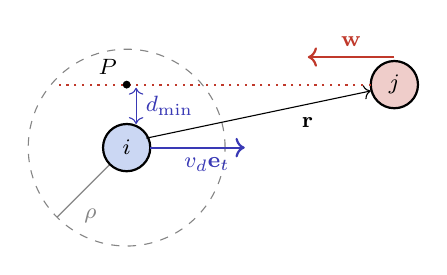
\begin{tikzpicture}[font=\footnotesize,scale=1.0]
        \draw[dashed,TPNavGray] (0,0) circle (1.25);
        \draw[TPNavGray] (0,0) -- node[pos=0.75,below right] {$\rho$} (-0.88,-0.88);
        \draw[thick,fill=TPFresca!25] (0,0) circle (0.3);
        \node at (0,0) {$i$};
        \draw[->,thick,TPBlue] (0.3,0) -- (1.5,0) node[below,pos=0.6] {$v_d\mathbf{e}_t$};
        \draw[thick,fill=TPUsada!25] (3.4,0.8) circle (0.3);
        \node at (3.4,0.8) {$j$};
        \draw[->] (0.25,0.12) -- (3.1,0.72) node[pos=0.65,below right] {$\mathbf{r}$};
        \draw[->,thick,TPUsada] (3.4,1.15) -- (2.3,1.15) node[above,pos=0.5] {$\mathbf{w}$};
        \draw[dotted,thick,TPUsada] (3.1,0.8) -- (-0.9,0.8);
        \fill (0,0.8) circle (0.05) node[above left] {$P$};
        \draw[<->,TPBlue] (0.12,0.3) -- (0.12,0.76) node[midway,right] {$d_{\min}$};
      \end{tikzpicture}
    \end{column}
  \end{columns}
  \vspace{2mm}
  \begin{itemize}\footnotesize\setlength{\itemsep}{1pt}
    \item \textbf{Esquema:} punteado, recorrido de $j$ visto desde $i$ (velocidad $\mathbf{w}$); $P$, máximo acercamiento, en $t^*$; círculo, $\rho$ alrededor de $i$
    \item $t_a$: horizonte de anticipación; $\rho$: espacio personal entre centros ($\rho = \rho_i + R$ de la teórica). Si deja de preverse el choque, vuelve a $\mathbf{x}_f$
    \item Diferencia con la Teórica 7: la velocidad de $i$ en la predicción es $v_d\,\mathbf{e}_t$, no $\mathbf{v}_i + \mathbf{F}_G\,\Delta t$
  \end{itemize}
\end{frame}

% 5 -- A y B, con esquema de x_T (Teórica 7, diapo 16: target temporal)
\begin{frame}{Capas A y B: lado y objetivo temporal}
  \setlength{\abovedisplayskip}{2pt}\setlength{\belowdisplayskip}{2pt}
  \begin{columns}[T,onlytextwidth]
    \begin{column}{0.56\textwidth}
      \begin{itemize}\small
        \item \textbf{Lado del desvío} $\sigma$
          \[ \sigma = \begin{cases} -\operatorname{sgn}(s_c) & |s_c| > \delta_s \\ -1\ (\text{derecha}) & |s_c| \le \delta_s \end{cases} \]
        \item \textbf{Objetivo temporal y dirección}
          \[ \mathbf{x}_T = \mathbf{x}_i + v_d\,t_a\,\mathbf{e}_t + \sigma\,\ell\,\mathbf{n} \]
          \[ \mathbf{e}_a = \frac{\mathbf{x}_T - \mathbf{x}_i}{|\mathbf{x}_T - \mathbf{x}_i|} \]
      \end{itemize}
    \end{column}
    \begin{column}{0.41\textwidth}
      \centering
      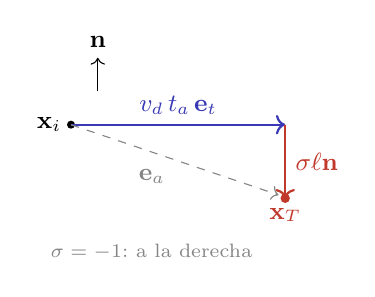
\begin{tikzpicture}[font=\small,scale=0.85]
        \fill (0,0) circle (0.06) node[left] {$\mathbf{x}_i$};
        \draw[->,thick,TPBlue] (0,0) -- (3.2,0) node[midway,above] {$v_d\,t_a\,\mathbf{e}_t$};
        \draw[->,thick,TPUsada] (3.2,0) -- (3.2,-1.1) node[midway,right] {$\sigma\ell\mathbf{n}$};
        \fill[TPUsada] (3.2,-1.1) circle (0.07) node[below] {$\mathbf{x}_T$};
        \draw[->,dashed,TPNavGray] (0,0) -- (3.1,-1.05) node[midway,below left] {$\mathbf{e}_a$};
        \draw[->,thin] (0.4,0.5) -- (0.4,1.0) node[above] {$\mathbf{n}$};
        \node[TPNavGray,font=\scriptsize] at (1.2,-1.9) {$\sigma = -1$: a la derecha};
      \end{tikzpicture}
      \begin{itemize}\scriptsize\setlength{\itemsep}{0pt}
        \item $\mathbf{n}$: normal izquierda de $\mathbf{e}_t$
        \item $s_c = \mathbf{n}\cdot(\mathbf{r}+\mathbf{w}t^*)$: lado de $j$ en $P$
        \item $\delta_s$: umbral de desempate
      \end{itemize}
    \end{column}
  \end{columns}
  \vspace{2mm}
  \begin{columns}[T,onlytextwidth]
    \begin{column}{0.48\textwidth}
      \begin{databox}{A: $(t_a,\ \ell)$}
        $\ell$: desvío lateral fijo (m)
      \end{databox}
    \end{column}
    \begin{column}{0.48\textwidth}
      \begin{databox}{B: $(t_a,\ k)$}
        $\ell = k\,(\rho - d_{\min})$; $k$: ganancia, sin unidades
      \end{databox}
    \end{column}
  \end{columns}
\end{frame}

% ---------------- IMPLEMENTACIÓN ----------------
\sectiondivider{Implementación}

% 8 -- Motor: lazo del paso temporal, con el estilo de «Arquitectura» de TP4
\begin{frame}[c]{Motor: paso temporal}
  \centering
  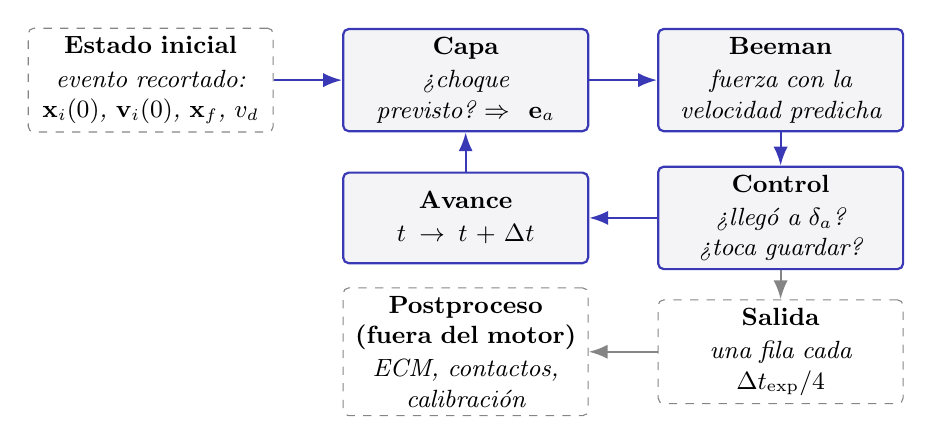
\begin{tikzpicture}[
      caja/.style={rectangle, rounded corners=2pt, draw=TPBlue, thick, fill=TPPlaceholder, align=center,
        minimum height=1.15cm, text width=2.9cm, font=\small, inner sep=3pt,
        execute at begin node=\hyphenpenalty10000\relax},
      externa/.style={rectangle, rounded corners=2pt, draw=TPNavGray, dashed, align=center,
        minimum height=1.15cm, text width=2.9cm, font=\small, inner sep=3pt,
        execute at begin node=\hyphenpenalty10000\relax},
      flecha/.style={-{Latex[length=2.4mm]}, draw=TPBlue, thick},
      flechagris/.style={-{Latex[length=2.4mm]}, draw=TPNavGray, thick},
      etiqueta/.style={font=\small, inner sep=2pt},
    ]
    \node[externa] (ic) at (0.0,2.1)  {\textbf{Estado inicial}\\[1pt]{\itshape evento recortado: $\mathbf{x}_i(0)$, $\mathbf{v}_i(0)$, $\mathbf{x}_f$, $v_d$}};
    \node[caja]    (ca) at (4.0,2.1)  {\textbf{Capa}\\[1pt]{\itshape ¿choque previsto? $\Rightarrow\ \mathbf{e}_a$}};
    \node[caja]    (be) at (8.0,2.1)  {\textbf{Beeman}\\[1pt]{\itshape fuerza con la velocidad predicha}};
    \node[caja]    (sa) at (8.0,0.35) {\textbf{Control}\\[1pt]{\itshape ¿llegó a $\delta_a$? ¿toca guardar?}};
    \node[caja]    (av) at (4.0,0.35) {\textbf{Avance}\\[1pt]{\itshape $t \to t + \Delta t$}};
    \node[externa] (out) at (8.0,-1.35) {\textbf{Salida}\\[1pt]{\itshape una fila cada $\Delta t_{\mathrm{exp}}/4$}};
    \node[externa] (me) at (4.0,-1.35) {\textbf{Postproceso (fuera del motor)}\\[1pt]{\itshape ECM, contactos, calibración}};
    \draw[flecha] (ic) -- (ca);
    \draw[flecha] (ca) -- (be);
    \draw[flecha] (be) -- (sa);
    \draw[flecha] (sa) -- (av);
    \draw[flecha] (av) -- (ca);
    \draw[flechagris] (sa) -- (out);
    \draw[flechagris] (out) -- (me);
  \end{tikzpicture}
  \par\vspace{2mm}
  {\small Beeman de TP4. $\Delta t_{\mathrm{exp}}$: tiempo entre cuadros de los datos. $\Delta t_{\mathrm{exp}}/32$ contra $/64$, con A(3;~0,5) y B(3,5;~1): el ECM 1 de cada evento cambia a lo sumo 0,18\,\%. Antes del recorte, con A(2,5;~2,5), el ECM 1 poblacional cambiaba 2,12\,\%: por eso se usa $/64$}
\end{frame}

% ---------------- SIMULACIONES ----------------
\sectiondivider{Simulaciones}

% 10 -- Recorte (animación + criterio)
\begin{frame}{Datos: recorte al tramo frontal}
  \begin{columns}[T,onlytextwidth]
    \begin{column}{0.62\textwidth}
      \videooimagen{figuras/anim-recorte.png}{3.4cm}{\animacionRecorteURL}{Animación del recorte (evento 11)}
      \par\vspace{1mm}
    \end{column}
    \begin{column}{0.35\textwidth}
      \parambox{
        \item Persistencia: 5 cuadros
        \item $X = 1{,}5$ m
        \item Animación: evento 11}
    \end{column}
  \end{columns}
  \begin{itemize}\scriptsize
    \item \textbf{Tramo D(45°):} cuadros comunes con los dos a $\le 45^\circ$ del eje $x$, en sentidos opuestos, en el bloque del mínimo real
    \item \textbf{Compuerta:} si un tramo pasa la $x$ inicial del otro por más de $X$, la ventana termina antes. $X$ se fijó después de ver los datos
    \item $\mathbf{x}_f$: última posición de la ventana común; $v_d$: rapidez media en esa ventana
  \end{itemize}
\end{frame}

% 11 -- Parámetros: dos columnas con viñetas, sin recuadros (formato de TP4)
\begin{frame}{Sistema: parámetros}
  \small
  \begin{columns}[T,onlytextwidth]
    \begin{column}{0.48\textwidth}
      \textbf{Fijos}
      \begin{itemize}[itemsep=1pt,topsep=2pt]
        \item $m = 80$~kg; $\tau = 0{,}5$~s; $R = 0{,}25$~m
        \item $k_n = 1{,}2\cdot 10^5$ N/m; $k_t = 2{,}4\cdot 10^5$ kg/(m s)
        \item $\rho = 0{,}9$ m; $\delta_s = 0{,}05$ m
        \item $\Delta t = \Delta t_{\mathrm{exp}}/64$; $\Delta t_{\mathrm{exp}} = 1/15{,}0192$ s
        \item Llegada: $\delta_a = 0{,}1$ m del objetivo
        \item $\mathbf{x}_i(0)$, $\mathbf{v}_i(0)$: de los datos ($\mathbf{v}_i(0)$: ajuste lineal de 5 cuadros)
      \end{itemize}
    \end{column}
    \begin{column}{0.48\textwidth}
      \textbf{Variables (grilla)}
      \begin{itemize}[itemsep=1pt,topsep=2pt]
        \item A: $t_a \in [0{,}5;\,5]$ s, paso 0,5; $\ell \in [0;\,2{,}5]$ m, paso 0,25 (110 pares)
        \item B: mismo $t_a$; $k \in [0;\,4]$, paso 0,5 (90 pares)
        \item Mejor par: mínimo de $\langle E\rangle$ en la grilla, por métrica
      \end{itemize}
    \end{column}
  \end{columns}
  \par\vspace{2mm}
  {\footnotesize Coeficientes del SFM: Teórica 6 y Helbing (2000); $R$: enunciado.}
\end{frame}

% 12 -- Observables
\begin{frame}{Observables y validación}
  \setlength{\abovedisplayskip}{2pt}\setlength{\belowdisplayskip}{2pt}
  \small
  \begin{columns}[T,onlytextwidth]
    \begin{column}{0.48\textwidth}
      \textbf{ECM 1} (mismo instante, m$^2$)
      \[ \scalebox{0.9}{$\displaystyle \mathrm{ECM}_1 = \frac{1}{N}\sum_{k=1}^{N} \left|\mathbf{x}^{\mathrm{sim}}(t_k) - \mathbf{x}^{\mathrm{exp}}(t_k)\right|^2$} \]
    \end{column}
    \begin{column}{0.50\textwidth}
      \textbf{ECM 2} (punto más cercano de la trayectoria simulada)
      \[ \scalebox{0.9}{$\displaystyle \mathrm{ECM}_2 = \frac{1}{N}\sum_{k=1}^{N} \min_{s}\left|\mathbf{x}^{\mathrm{exp}}(t_k) - \mathbf{x}^{\mathrm{sim}}(s)\right|^2$} \]
    \end{column}
  \end{columns}
  \begin{itemize}\footnotesize
    \item \textbf{Por peatón;} $t_k$: sus $N$ cuadros en la ventana (sin los faltantes); ECM 1 excluye los posteriores a la llegada. $E_m$: promedio de los 2 peatones; $\langle E\rangle$: promedio de los eventos
    \item \textbf{Distancia entre peatones} $d(t) = |\mathbf{x}_1 - \mathbf{x}_2|$ (entre centros); $D^{\mathrm{exp}}$, $D^{\mathrm{sim}}$: su mínimo, real y simulado
    \item \textbf{Corrimiento del mínimo:} $c = t(D^{\mathrm{sim}}) - t(D^{\mathrm{exp}})$; ``llega tarde'' si $c > 0$. \textbf{Contacto:} $\varepsilon_{ij} < 0$ en algún paso
    \item \textbf{Calibración individual:} el par que minimiza $E_m$ en cada evento.
    \item \textbf{Validación:} particiones al azar en calibración y validación; $\pm$: desvío entre particiones
  \end{itemize}
\end{frame}

% ---------------- RESULTADOS ----------------
\sectiondivider{Resultados}

% 14 -- Animaciones (punto a)
\begin{frame}{Animaciones: sin capa, A y B}
      \par{\footnotesize Sin capa y A(3; 0,5) [Evento 16]}\par
      \videooimagen{figuras/anim-sin-capa-vs-A.png}{2.5cm}{\animacionSinCapaURL}{Sin capa y A}
      \par\vspace{1mm}{\footnotesize A y B con su mejor par de ECM 1 [Evento 16]}\par
      \videooimagen{figuras/anim-A-B.png}{2.5cm}{\animacionURL}{A y B}
\end{frame}

% 15 -- Observable primario en el tiempo
\begin{frame}[c]{Distancia entre peatones en el tiempo}
  \resultadofigura{figuras/T1-distancia-vs-t.pdf}{6.0cm}{Distancia entre peatones vs t (evento 16)}
    {\item Evento 16
     \item Mejor par de ECM 1 de cada capa}{}{}
  \par\vspace{2mm}
  \begin{center}
    \small\renewcommand{\arraystretch}{1.15}
    \begin{tabular}{@{}lcc@{}}
      \hline
      & $D$ (m) & Corrimiento $c$ (s) \\ \hline
      Real ($D^{\mathrm{exp}}$) & 0,68 & --- \\
      A(3; 0,5) & 0,61 & $+0{,}26$ \\
      B(3,5; 1) & 0,56 & $+0{,}28$ \\ \hline
    \end{tabular}
  \end{center}
\end{frame}

% 16 -- Calibración poblacional (punto b): mapas de las dos métricas
\newcommand{\mapados}[3]{%
  {\footnotesize Cada celda: error poblacional $\langle E\rangle$ (#2, promedio de los 19 eventos) con ese par. Más claro = menos error. Fila $\ell = 0$ o $k = 0$: la capa no desvía y el error es el de sin capa}
  \par\vspace{1mm}
  \begin{columns}[T,onlytextwidth]
    \begin{column}{0.49\textwidth}\centering\maybeimage{figuras/R2-A-#1.pdf}{4.1cm}{A, #2}\par{\small A: $(t_a,\ \ell)$}\end{column}
    \begin{column}{0.49\textwidth}\centering\maybeimage{figuras/R2-B-#1.pdf}{4.1cm}{B, #2}\par{\small B: $(t_a,\ k)$}\end{column}
  \end{columns}
  \par\vspace{1mm}
  {\footnotesize Color: $\langle E\rangle$ (#2) de cada par de la grilla. Estrella: óptimo de #2; círculo vacío: óptimo de #3}%
}
\begin{frame}{Calibración poblacional: ECM 1 en la grilla}
  \mapados{ecm1}{ECM 1}{ECM 2}
\end{frame}

\begin{frame}{Calibración poblacional: ECM 2 en la grilla}
  \mapados{ecm2}{ECM 2}{ECM 1}
\end{frame}

% 17 -- Mejores pares y validación cruzada (puntos b y d)
\begin{frame}[c]{Mejor par de cada capa y validación cruzada}
  \resultadofigura{figuras/M1-mejores-pares.pdf}{6.0cm}{ECM 1 y ECM 2 del mejor par, y ECM 1 de validación}
    {\item 5000 particiones: 14 eventos para calibrar y 5 para validar
     \item Semilla 20261116
     \item Sin capa no tiene parámetros: no hay validación}{}{}
\end{frame}

% 18 -- Calibración individual (punto c): óptimos
\begin{frame}{Calibración individual: dónde cae el óptimo de cada evento}
  \noindent{\footnotesize Para cada evento, el par de la grilla que minimiza su $E_m$ (ECM 1). Número en la celda: cuántos eventos tienen ahí su óptimo. Recuadro negro: óptimo poblacional. ECM 2, en el anexo}
  \par\vspace{1mm}
  \begin{columns}[T,onlytextwidth]
    \begin{column}{0.49\textwidth}\centering\maybeimage{figuras/C1-conteo-A-ecm1.pdf}{4.9cm}{Óptimos individuales, A, ECM 1}\par{\small A: $(t_a,\ \ell)$}\end{column}
    \begin{column}{0.49\textwidth}\centering\maybeimage{figuras/C1-conteo-B-ecm1.pdf}{4.9cm}{Óptimos individuales, B, ECM 1}\par{\small B: $(t_a,\ k)$}\end{column}
  \end{columns}
\end{frame}

% 19 -- Calibración individual (punto c): ganancia
\begin{frame}{Calibración individual: cuánto se gana}
  \noindent{\footnotesize Distribución de $E_m$ en los 19 eventos: con el par poblacional (lleno) y con el mejor par de cada evento (vacío). Arriba: cambio de la media}
  \par\vspace{1mm}
  \begin{columns}[T,onlytextwidth]
    \begin{column}{0.49\textwidth}
      \centering\maybeimage{figuras/C2-ecm1.pdf}{4.9cm}{$E_m$ poblacional vs individual, ECM 1}
      \par{\small ECM 1}
    \end{column}
    \begin{column}{0.49\textwidth}
      \centering\maybeimage{figuras/C2-ecm2.pdf}{4.9cm}{$E_m$ poblacional vs individual, ECM 2}
      \par{\small ECM 2}
    \end{column}
  \end{columns}
\end{frame}

% ---------------- CONCLUSIONES ----------------
\sectiondivider{Conclusiones}

% 21
\begin{frame}{Conclusiones}
  \footnotesize
  \begin{itemize}\setlength{\itemsep}{0pt}
    \item \textbf{Efecto de la capa:} sin capa hay contacto en los 19 eventos y ECM 1 de 3,18 m$^2$; con A y B, ningún contacto y ECM 1 de 0,43 y 0,41 m$^2$ (par de ECM 1, $\rho = 0{,}9$ m)
    \item \textbf{A frente a B:} casi no se distinguen (validación de ECM 1: 0,451 y 0,422 m$^2$, $\pm$ 0,10). B depende más de $\rho$ (anexo); su óptimo es el mismo en ECM 1 y ECM 2, (3,5; 1); el de A cambia con la métrica, (3; 0,5) y (2; 0,5)
    \item \textbf{Calibración individual:} casi nunca coincide el óptimo individual con el poblacional (A: 1 de 19; B: 2 de 19). Baja la media de $E_m$: ECM 1, 5,5 y 2,6\,\% (A, B); ECM 2, 31,9 y 28,1\,\%
    \item \textbf{Límite:} A y B llegan tarde al mínimo (mediana de $c$: $+0{,}40$ y $+0{,}41$ s; anexo). No lo causa la capa: sin capa el atraso es el mismo. Causa probable: la relajación de $\mathbf{v}_i(0)$ hacia $v_d$ ($\tau = 0{,}5$ s)
    \item \textbf{Elección:} \textcolor{TPUsada}{\textbf{[completar]}}
  \end{itemize}
\end{frame}

% 22
\begin{frame}{Uso de IA}
  \begin{itemize}
    \item Agentes: Claude (Sonnet 5.5) para plan; Claude Code (claude-opus-5-5) para el motor
    \item El grupo revisó cada etapa con tests y verificó visualmente los 19 recortes
  \end{itemize}
\end{frame}

% 23
\begin{frame}{}
  \vfill
  \begin{beamercolorbox}[wd=0.86\paperwidth,ht=0.72cm,dp=0.20cm,center]{frametitle}
    \LARGE Muchas gracias
  \end{beamercolorbox}
  \vspace{0.4cm}
  \begin{center}\maybeimage{figuras/muchas_gracias.jpeg}{3.1cm}{Insertar imagen de cierre}\end{center}
  \vfill
\end{frame}

% ---------------- ANEXO ----------------
% 24
\begin{frame}{Anexo: Consultas a la cátedra}
  \small
  \begin{itemize}
    \item \textbf{Recorte:} ¿es válido el criterio D(45°) más una regla de compuerta fijada después de ver los datos?
    \item \textbf{Objetivo final:} ¿$\mathbf{x}_f$ y $v_d$ de la ventana común, o el final del propio tramo de cada peatón?
    \item \textbf{Retraso:} ¿es esperable que las capas lleguen tarde al mínimo?
    \item \textbf{$\rho$ y B:} B con $\rho = 0{,}9$ (cerca del máximo de las distancias mínimas reales, 0,92 m) ¿es un criterio razonable para fijar $\rho$?
    \item \textbf{Predicción:} ¿vale usar $v_d\,\mathbf{e}_t$ como velocidad de $i$ en vez de $\mathbf{v}_i + \mathbf{F}_G\,\Delta t$ (Teórica 7)?
    \item \textbf{$v_d$:} ¿constante, o seguir el perfil de rapidez real? Los peatones de la derecha van $+0{,}21$ m/s sobre $v_d$ antes del mínimo y $-0{,}18$ m/s después (medianas)
    \item \textbf{Regla de lado:} en A acierta el lado en 14 de 19 eventos, igual que ``siempre a la derecha''. ¿Es aceptable?
  \end{itemize}
\end{frame}


% F (descartada): definición, mapas y diferencias por evento
\begin{frame}{Anexo: capa F (descartada), definición}
  \setlength{\abovedisplayskip}{2pt}\setlength{\belowdisplayskip}{2pt}
  \begin{itemize}\small
    \item \textbf{Repulsión direccional}
      \[ \mathbf{n}_c = \mathbf{e}_{ij}\,A_p\,e^{-d_{ij}/B_p}\cos\theta_j \qquad (\cos\theta_j > 0) \]
    \item \textbf{Dirección deseada}
      \[ \mathbf{e}_a = \frac{\mathbf{n}_c + \mathbf{e}_t}{|\mathbf{n}_c + \mathbf{e}_t|} \]
  \end{itemize}
  \begin{itemize}\footnotesize\setlength{\itemsep}{1pt}
    \item $\mathbf{e}_{ij}$: versor de $j$ a $i$; $d_{ij}$: distancia entre centros; $\cos\theta_j = \mathbf{e}_t\cdot(\mathbf{x}_j - \mathbf{x}_i)/d_{ij}$: solo ve $j$ adelante (semiplano)
    \item $A_p \in (0,1)$: intensidad, sin unidades; $B_p$: alcance (m)
    \item Choque casi frontal ($|s_c| \le \delta_s$): $\mathbf{e}_{ij}$ rotado un ángulo $\theta_d$ para desviar a la derecha; si no alcanza, $-\mathbf{e}_t$ rotado $\theta_d$
    \item \textbf{Grilla:} $A_p \in [0{,}1;\,0{,}9]$, paso 0,1; $B_p \in \{0{,}25;\,0{,}5;\,0{,}75;\,1;\,1{,}5;\,2;\,2{,}5;\,3\}$ m (72 pares); $\theta_d = 5^\circ$
    \item \textbf{Diferencias con la Teórica 7:} solo actúa con choque previsto (sin horizonte); sigue activa durante el contacto; cambia $\mathbf{e}_a$ directamente, sin objetivo temporal $\mathbf{x}_T$
  \end{itemize}
\end{frame}

\begin{frame}{Anexo: capa F, ECM en la grilla}
  \begin{columns}[T,onlytextwidth]
    \begin{column}{0.49\textwidth}\centering\maybeimage{figuras/R2-F-ecm1.pdf}{4.6cm}{F, ECM 1}\par{\small ECM 1}\end{column}
    \begin{column}{0.49\textwidth}\centering\maybeimage{figuras/R2-F-ecm2.pdf}{4.6cm}{F, ECM 2}\par{\small ECM 2}\end{column}
  \end{columns}
  \par\vspace{1mm}
  {\footnotesize Color: $\langle E\rangle$ de cada par $(A_p, B_p)$. Estrella: óptimo de la métrica del mapa; círculo vacío: óptimo de la otra. Mejor par: (0,9; 3) en ECM 1 y (0,8; 3) en ECM 2, en el borde de la grilla}
\end{frame}

% 31
\begin{frame}[c]{Anexo: capa F frente a A y B}
  \resultadofigura{figuras/M1-mejores-pares-con-F.pdf}{6.0cm}{ECM 1 y ECM 2 del mejor par, y ECM 1 de validación, con F}
    {\item 5000 particiones: 14 eventos para calibrar y 5 para validar
     \item F: contacto en 17 de 19 eventos}{}{}
\end{frame}

\begin{frame}{Anexo: diferencias por evento con F}
  \begin{columns}[T,onlytextwidth]
    \begin{column}{0.73\textwidth}
      \centering
      \maybeimage{figuras/R4b-pareadas.pdf}{3.2cm}{Diferencia de ECM 1 por evento, F $-$ A}\par\vspace{1mm}
      \maybeimage{figuras/R4c-pareadas.pdf}{3.2cm}{Diferencia de ECM 1 por evento, F $-$ B}
    \end{column}
    \begin{column}{0.25\textwidth}
      \parambox{\item Mejor par de ECM 1 de cada capa
        \item Barra hacia arriba: gana A (arriba) o B (abajo)}
    \end{column}
  \end{columns}
\end{frame}

% 26
\begin{frame}[c]{Anexo: A elige el lado de cruce contrario al real (evento 12)}
  \animacionsimple{figuras/anim-lado-evento12.png}{5.0cm}{\animacionLadoURL}{Evento 12: real y A}
    {\item Evento 12
     \item A(3; 0,5)}
  \par\vspace{1mm}
  {\footnotesize En el evento 12 los peatones reales se cruzan dejando al otro a su derecha (pasan por su izquierda); con A, la regla de lado los desvía a su derecha y se cruzan del otro lado. Pasa en 5 de 19 eventos (6, 8, 10, 12 y 17)}
\end{frame}

\begin{frame}{Anexo: calibración individual en ECM 2}
  \noindent{\footnotesize Igual que en Resultados, con ECM 2: número en la celda, cuántos eventos tienen ahí su óptimo; recuadro negro, óptimo poblacional de ECM 2}
  \par\vspace{1mm}
  \begin{columns}[T,onlytextwidth]
    \begin{column}{0.49\textwidth}\centering\maybeimage{figuras/C1-conteo-A-ecm2.pdf}{4.9cm}{Óptimos individuales, A, ECM 2}\par{\small A: $(t_a,\ \ell)$}\end{column}
    \begin{column}{0.49\textwidth}\centering\maybeimage{figuras/C1-conteo-B-ecm2.pdf}{4.9cm}{Óptimos individuales, B, ECM 2}\par{\small B: $(t_a,\ k)$}\end{column}
  \end{columns}
\end{frame}

% 27
\begin{frame}[c]{Anexo: validación cruzada por partición}
  \resultadofigura{figuras/R3-validacion.pdf}{5.6cm}{ECM 1 de validación de cada partición}
    {\item 5000 particiones
     \item 14 eventos para calibrar y 5 para validar
     \item Semilla 20261116}{}{}
  \par\vspace{1mm}
  {\scriptsize Control de convergencia (media de validación): 2500 contra 5000 particiones cambia menos de 1\,\% (a lo sumo 0,57\,\%); 1000 contra 5000 no pasa en A y B (hasta 1,71\,\%).}
\end{frame}

% 28
\begin{frame}{Anexo: distancia mínima y corrimiento}
  \begin{columns}[T,onlytextwidth]
    \begin{column}{0.49\textwidth}
      \centering\maybeimage{figuras/R5-distancia-minima.pdf}{5.0cm}{$D^{\mathrm{sim}}$ vs $D^{\mathrm{exp}}$}
    \end{column}
    \begin{column}{0.49\textwidth}
      \centering\maybeimage{figuras/R5b-corrimiento.pdf}{5.0cm}{Corrimiento $c$ por evento}
    \end{column}
  \end{columns}
  \par\vspace{1mm}
  {\footnotesize Mejor par de ECM 1 de cada capa: A(3; 0,5) y B(3,5; 1). Izquierda: debajo de la identidad, el simulado pasa más cerca que el real. Derecha: $c > 0$, llega tarde}
\end{frame}

% 29
\begin{frame}[c]{Anexo: robustez frente a $\rho$}
  \resultadofigura{figuras/R6-robustez-rho.pdf}{5.0cm}{Variación del ECM 1 según $\rho$ para A y B}
    {\item $\rho \in [0{,}7;\,1{,}1]$ m
     \item A(3; 0,5) y B(3,5; 1) fijos}{}{}
\end{frame}

% 30
\begin{frame}[c]{Anexo: diferencias por evento entre A y B}
  \resultadofigura{figuras/R4-pareadas.pdf}{6.0cm}{Diferencia de ECM 1 por evento, A $-$ B}
    {\item Mejor par de ECM 1 de cada capa
     \item Barra hacia arriba: gana B}{}{}
\end{frame}

% 32
\begin{frame}[c]{Anexo: sensibilidad a la velocidad inicial}
  \resultadofigura{figuras/V0-sensibilidad.pdf}{5.5cm}{ECM 1 con $v_0$ de 3, 5 y 7 cuadros}
    {\item $v_0$: ajuste lineal de los primeros cuadros del tramo
     \item $\rho = 0{,}9$ m}{}{}
\end{frame}

% 33--35: tabla de correcciones (Notion "Correcciones a la IA" + docs/ia/correcciones.md)
\newcommand{\corrhead}{\hline \textbf{Fecha} & \textbf{Qué hizo la IA} & \textbf{Corrección} \\ \hline}
\begin{frame}{Anexo: Correcciones a la IA (1/2)}
  \scriptsize\renewcommand{\arraystretch}{1.3}
  \begin{tabular}{@{}p{0.9cm}p{5.2cm}p{4.75cm}@{}}
    \corrhead
    3/11 & Recomendó que el peatón se detenga al llegar al objetivo & Sigue a $v_d$ y se retira a 0,1 m del objetivo \\
    3/11 & Recomendó diferencia central para la velocidad inicial & Ajuste lineal de 5 cuadros, igual para ambos \\
    3/11 & Test del ECM 1 esperaba 4; el correcto era 2,6 & Se corrigió el test, no el motor \\
    4/11 & Planteó, sin verificarlo, que el 455\% del evento 2 era un contacto & Era un cambio de lado; el contacto era del evento 17 \\
    4/11 & Dio por cumplido el ``evita oscilar'' de la especificación & Oscila por el umbral $\rho$; se declaró \\
    5/11 & Dio por validado $\Delta t_{\mathrm{exp}}/32$ sin probar con capas & Con A(2,5; 2,5), sin recorte, el ECM 1 poblacional cambia 2,12\% entre $/32$ y $/64$; se pasó a $/64$ \\
    \hline
  \end{tabular}
\end{frame}
\begin{frame}{Anexo: Correcciones a la IA (2/2)}
  \scriptsize\renewcommand{\arraystretch}{1.3}
  \begin{tabular}{@{}p{0.9cm}p{5.2cm}p{4.75cm}@{}}
    \corrhead
    11/11 & Fijó el objetivo y $v_d$ con la trayectoria completa & Lo detectó la cátedra (Franco): se recortó al tramo frontal \\
    11/11 & Referencia lateral contaminada por el tramo vertical; rumbo máximo contaminado por la salida & Se corrigieron los cálculos \\
    11/11 & Recorte que no era idempotente; caso sintético mal armado en un test & Se corrigieron el recorte y el test \\
    11/11 & Recomendó D(45°), que deja la cola izquierda en los eventos 3 y 6 & Lo detectó la verificación visual del grupo; se agregó la compuerta \\
    12/11 & Rotuló ``Postproceso (fuera del motor)'' con el ECM, los contactos y la grilla todavía en el motor & Se volvió a ``Después de la corrida''; con \texttt{analysis/} fuera del ZIP, el rótulo pasó a ser cierto \\
    12/11 & Propuso calcular el ECM y los contactos dentro del motor de la entrega & Se separaron del motor (penalización del TP4); 258/258 archivos de salida idénticos \\
    \hline
  \end{tabular}
\end{frame}

\end{document}
